\documentclass{article}
\usepackage{amsmath}
\usepackage{tikz}
\usetikzlibrary{arrows.meta}

\begin{document}

\begin{figure}[h]
    \centering
    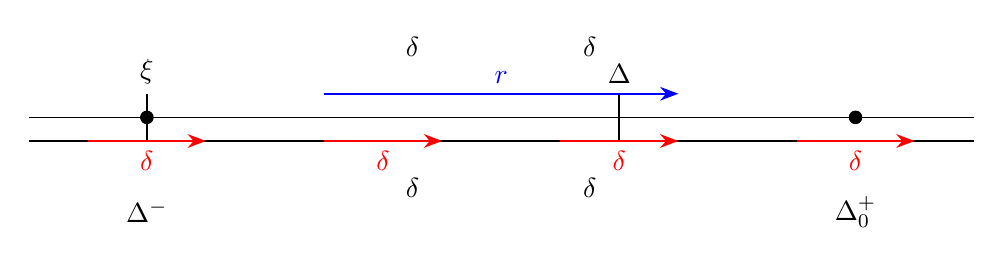
\begin{tikzpicture}[scale=1.5, >=Stealth]
        % Draw the horizontal line segment
        \draw[black] (-4,0) -- (4,0);
        
        % Label the segments
        \draw[thick] (-3,-0.2) -- (-3,0.2) node[above] {$\xi$};
        \draw[thick] (1,-0.2) -- (1,0.2) node[above] {$\Delta$};
        
        % Draw the vertical line segment
        \draw[thick] (-4,-0.2) -- (4,-0.2);
        
        % Mark the points with delta
        \filldraw[black] (-3,0) circle (1.5pt);
        \filldraw[black] (3,0) circle (1.5pt);
        
        % Labels for delta
        \node at (-3,-0.8) {$\Delta^{-}$};
        \node at (3,-0.8) {$\Delta_{0}^{+}$};
        
        % Blue arrows for r
        \draw[blue, thick, -Stealth] (-1.5,0.2) -- (1.5,0.2) node[midway, above] {$r$};
        
        % Red arrows for delta
        \draw[red, thick, -Stealth] (-3.5,-0.2) -- (-2.5,-0.2) node[midway, below] {$\delta$};
        \draw[red, thick, -Stealth] (-1.5,-0.2) -- (-0.5,-0.2) node[midway, below] {$\delta$};
        \draw[red, thick, -Stealth] (0.5,-0.2) -- (1.5,-0.2) node[midway, below] {$\delta$};
        \draw[red, thick, -Stealth] (2.5,-0.2) -- (3.5,-0.2) node[midway, below] {$\delta$};
        
        % Additional labels
        \node at (-0.75,0.6) {$\delta$};
        \node at (0.75,0.6) {$\delta$};
        
        \node at (-0.75,-0.6) {$\delta$};
        \node at (0.75,-0.6) {$\delta$};
    \end{tikzpicture}
    
    \caption{Schematic picture of $\Delta, \Delta^-, \Delta_0, \Delta^+$. We will usually take $r = \frac{\tau}{2n}$ and $\delta = \frac{1}{2m}$ for $n \ll m$, for example, later in the paper we use $m = n^{1 + \beta'}$ below.}
    \label{fig:delta_diagram}
\end{figure}

\end{document}